% Theorems
\newtheorem{theorem}{Теорема}
\newtheorem{statement}[theorem]{Утверждение}

\theoremstyle{definition}
\newtheorem{example}{Пример}
%-------------------------------------------------------------------------------
% New commands
\newcommand{\Zfull}{[\mathcal Z^{(1)} + 2\mathcal Z^{(2)}]}
\newcommand{\Zone}{\mathcal Z^{(1)}}
\newcommand{\Ztwo}{\mathcal Z^{(2)}}

\newcommand{\HB}{H\mathcal B}
\newcommand{\HSet}{HSet}
%-------------------------------------------------------------------------------
% New draw commands
\newcommand{\dA}{
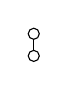
\begin{tikzpicture}
\draw (0pt,2pt) -- (0pt,6pt);
\draw (0pt,0pt) circle (2pt);
\draw (0pt,8pt) circle (2pt);
\end{tikzpicture}
} 

\newcommand{\dB}{
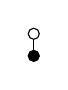
\begin{tikzpicture}
\draw (0pt,2pt) -- (0pt,6pt);
\draw[fill] (0pt,0pt) circle (2pt);
\draw (0pt,8pt) circle (2pt);
\end{tikzpicture}
} 

\newcommand{\dAA}{
\begin{tikzpicture}
\draw (0pt,0pt) -- (0pt,8pt);
\draw (0pt,0pt) -- (8pt,0pt);
\draw (8pt,8pt) -- (0pt,8pt);
\draw (8pt,8pt) -- (8pt,0pt);
\end{tikzpicture}
} 

\newcommand{\dBB}{

\begin{tikzpicture}
\draw[line width=1.5pt] (0pt,0pt) -- (0pt,8pt);
\draw[line width=1.5pt] (0pt,0pt) -- (8pt,0pt);
\draw (8pt,8pt) -- (0pt,8pt);
\draw (8pt,8pt) -- (8pt,0pt);
\end{tikzpicture}
} 